% !TEX TS-program = pdflatex
% !TEX encoding = UTF-8 Unicode

% This is a simple template for a LaTeX document using the "article" class.
% See "book", "report", "letter" for other types of document.

\documentclass[8pt]{article} % use larger type; default would be 10pt

\usepackage[utf8]{inputenc} % set input encoding (not needed with XeLaTeX)
\usepackage{bchart}
\usepackage{longtable}
\usepackage{pgfgantt}
\usepackage{calendar} % Use the calendar.sty style
\usepackage{calc}
\usepackage{ifthen}
\usepackage{tkz-base}
\usepackage{pdfpages}
\usepackage{hyperref}
\usepackage{pgfplots}
\usepackage{tkz-kiviat,numprint,fullpage} 
\usepackage{pgfplotstable} 
\usetikzlibrary{arrows}
\usepackage{paralist} % very flexible & customisable lists (eg. enumerate/itemize, etc.)
\usepackage{dcolumn}
\usepackage{booktabs}
\usepackage{lscape}
\usepackage{pgf-pie}
\usepackage{verbatim}
\usepackage{animate}
\usepackage{sfmath}

%%% Examples of Article customizations
% These packages are optional, depending whether you want the features they provide.
% See the LaTeX Companion or other references for full information.

\usepackage{textcomp}
%\usepackage{hyperref}

%%% PAGE DIMENSIONS
\usepackage{geometry} % to change the page dimensions
\geometry{a4paper} % or letterpaper (US) or a5paper or....
% \geometry{margin=2in} % for example, change the margins to 2 inches all round
% \geometry{landscape} % set up the page for landscape
%   read geometry.pdf for detailed page layout information

\usepackage{graphicx} % support the \includegraphics command and options

% \usepackage[parfill]{parskip} % Activate to begin paragraphs with an empty line rather than an indent

%%% PACKAGES
\usepackage{booktabs} % for much better looking tables
\usepackage{array} % for better arrays (eg matrices) in maths
\usepackage{paralist} % very flexible & customisable lists (eg. enumerate/itemize, etc.)
\usepackage{verbatim} % adds environment for commenting out blocks of text & for better verbatim
\usepackage{subfig} % make it possible to include more than one captioned figure/table in a single float
% These packages are all incorporated in the memoir class to one degree or another...

%%% HEADERS & FOOTERS
\usepackage{fancyhdr} % This should be set AFTER setting up the page geometry
\pagestyle{fancy} % options: empty , plain , fancy
\renewcommand{\headrulewidth}{0pt} % customise the layout...
\lhead{}\chead{}\rhead{}
\lfoot{}\cfoot{\thepage}\rfoot{}

%%% SECTION TITLE APPEARANCE
\usepackage{sectsty}
\allsectionsfont{\sffamily\mdseries\upshape} % (See the fntguide.pdf for font help)
% (This matches ConTeXt defaults)

%%% ToC (table of contents) APPEARANCE
\usepackage[nottoc,notlof,notlot]{tocbibind} % Put the bibliography in the ToC
\usepackage[titles,subfigure]{tocloft} % Alter the style of the Table of Contents
\renewcommand{\cftsecfont}{\rmfamily\mdseries\upshape}
\renewcommand{\cftsecpagefont}{\rmfamily\mdseries\upshape} % No bold!

%%% END Article customizations

%%% The "real" document content comes below...

%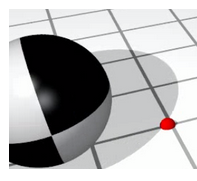
\includegraphics[width=.2\textwidth]{Logo.png}

\title{Finance}
\author{\copyright Frederic Kerdraon}
%\date{} % Activate to display a given date or no date (if empty),
         % otherwise the current date is printed 

%\addtobeamertemplate{frametitle}{}{%
%\begin{tikzpicture}[remember picture,overlay]
%\node[anchor=north west,yshift=2pt] at (current page.north west) {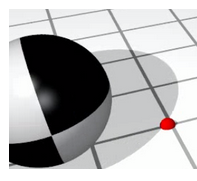
\includegraphics[height=0.8cm]{Logo1}};
%\end{tikzpicture}}

\begin{document}
\maketitle
\tableofcontents

%%%%%%%%%%%%%%%%%%%%%%%%%%%%%%%%%%%%%%%%%%%%%%%%%%%%%%%%%%%%%%%%%%%%%%%%%%%%%%%%%%%%%%%%%%%%%%%%%%%%%%%%%%%%%%%%%%%%%%%%%%%%%%%%%%%%%%%%%%%%%%%%%%%%%%%%%%%%%%
\section{Cash Balance Management}

\subsection{Monthly drift}

\subsubsection{Table}
%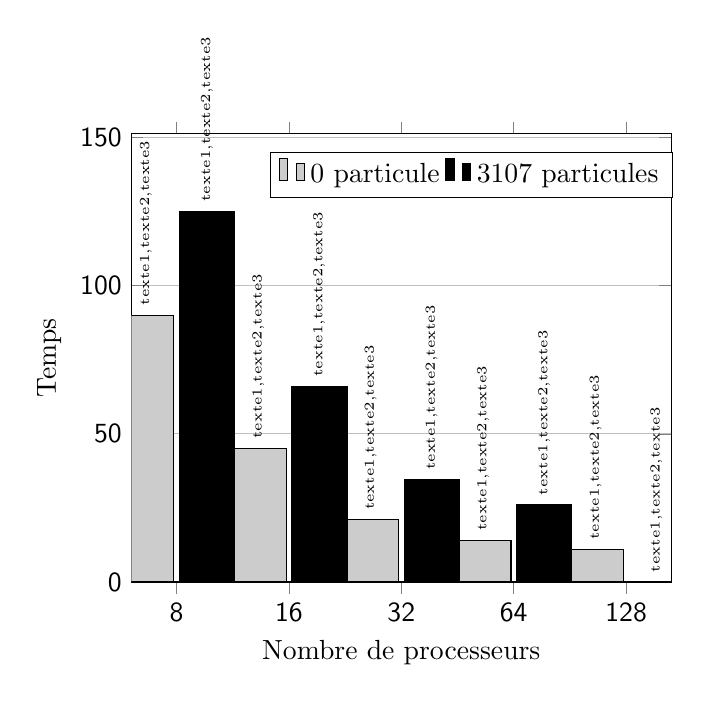
\begin{tikzpicture} \begin{axis}[
    x tick label style={
        /pgf/number format/1000 sep=},
    ymajorgrids,
    ylabel=Temps,
    xlabel= Nombre de processeurs,
    nodes near coords={texte1,texte2,texte3},
    xtick={1,2,3,4,5},
    xticklabels={$8$,$16$,$32$,$64$,$128$},
    enlarge y limits={upper,value=0.21},
    legend style={at={(0.63,0.96)},
        anchor=north,legend columns=-1},
    ybar,
    every node near coord/.append style={rotate=90, anchor=west,font=\tiny},
    bar width=20pt,
]
\addplot [ybar,fill=gray!40]
    coordinates {(1,90) (2,45)
         (3,21) (4,14) (5,11)};
\addplot [ybar,fill=black]
    coordinates {(1,125) (2,66)
        (3,34.5) (4,26) (5,0)};
\legend{0 particule,3107 particules,temps th\'eorique}
\end{axis}
\end{tikzpicture}

\begin{tikzpicture}[thick,scale=1.2]
\begin{axis}[
title={Cash over time},
xlabel={Time [Days]},
ylabel={Cash [euro]},
xmin=0,xmax=0,
ymin=0,ymax=0,
xtick={0,0,0,0,0},
ytick={0,0,0,0,0},
legend pos=north west,
ymajorgrids=true,
grid style=dashed,
]
\addplot[
color=blue,
mark=*,
]
coordinates {

};
\legend{Cash}
\end{axis}
\end{tikzpicture}


\subsubsection{Graph}
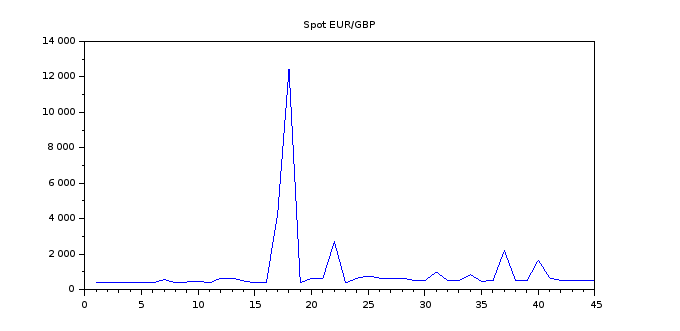
\includegraphics[scale=0.6]{Vector.png}

This where science enter the game as here can call scilab and there is no limit at what we could calculate... fascinating!
How do we populate Scilab with Negative numbers where there are Debits and Positive numbers for the Credit
\subsubsection{Graph}
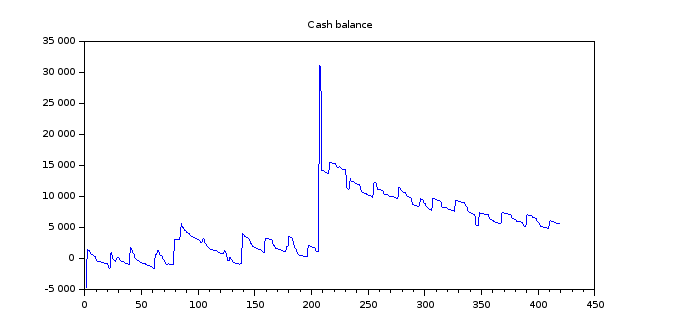
\includegraphics[scale=0.6]{Scilab-cashBalance.png}

\subsubsection{Map Of The Charges}
%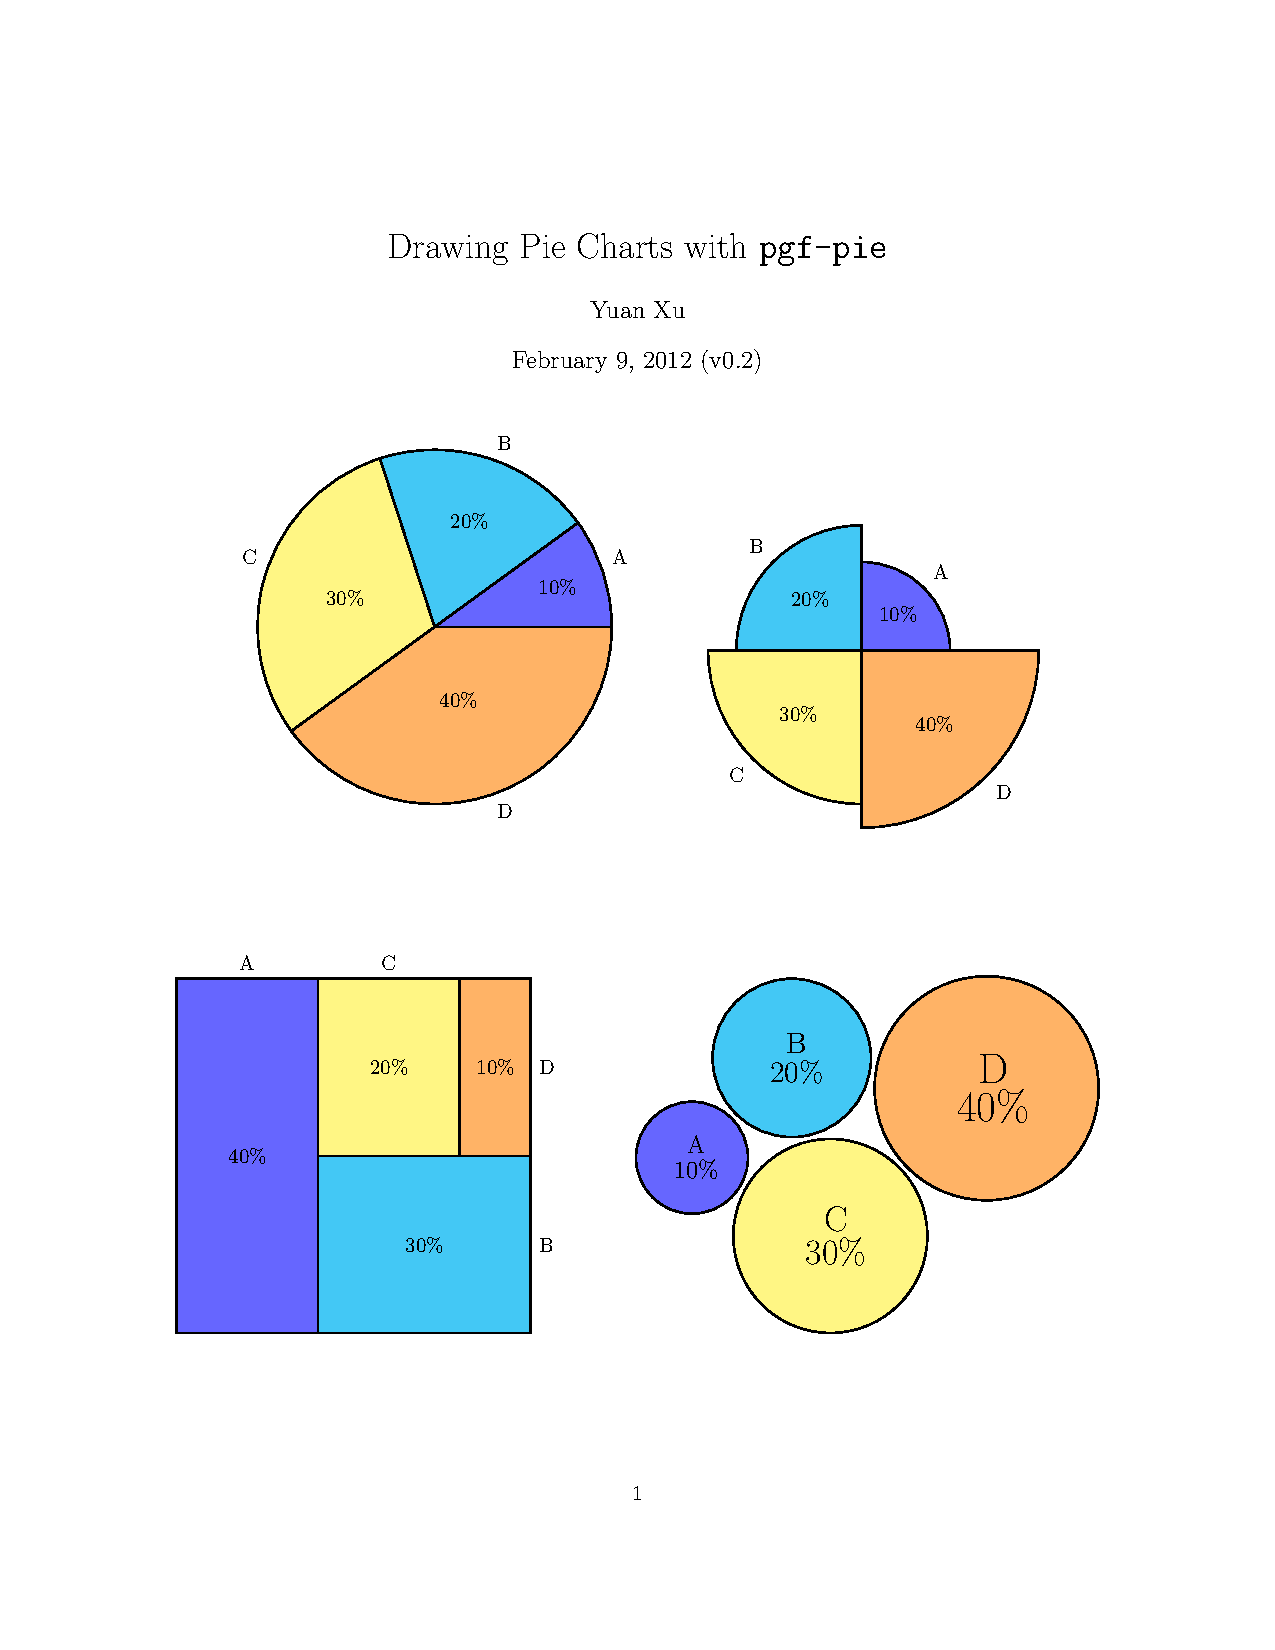
\includepdf[pages={1}]{MapOfTheCharges.pdf}
%\centering

%\begin{tikzpicture}[scale=0.5]
%\pie{13/A, 27/B, 30/C, 35/D}
%\end{tikzpicture}
%
\hspace{1cm}
%
%\begin{tikzpicture}[scale=0.5]
%  \pie[polar]{10/A, 20/B, 30/C, 40/D}
%\end{tikzpicture}

%\vspace{2cm}

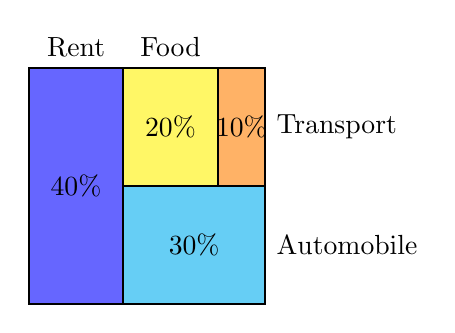
\begin{tikzpicture}[scale=0.5]
  \pie[square]{40/Rent, 30/Automobile, 20/Food, 10/Transport}
\end{tikzpicture}
%
\hspace{1cm}
%
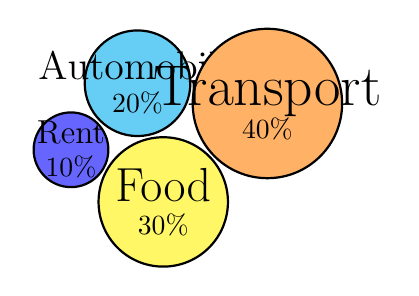
\begin{tikzpicture}[scale=0.5]
  \pie[cloud, text=inside, scale font]{10/Rent, 20/Automobile, 30/Food, 40/Transport}
\end{tikzpicture}


\subsubsection{Cash curve}
Funny cashflow/kapital superior to percent\\
\begin{tikzpicture}[thick,scale=1.2]
\begin{axis}[
title={Cash over time},
xlabel={Time [Days]},
ylabel={Cash [euro]},
xmin=0,xmax=0,
ymin=0,ymax=0,
xtick={0,0,0,0,0},
ytick={0,0,0,0,0},
legend pos=north west,
ymajorgrids=true,
grid style=dashed,
]
\addplot[
color=blue,
mark=*,
]
coordinates {

};
\legend{Cash}
\end{axis}
\end{tikzpicture}

%Checklists.tex:%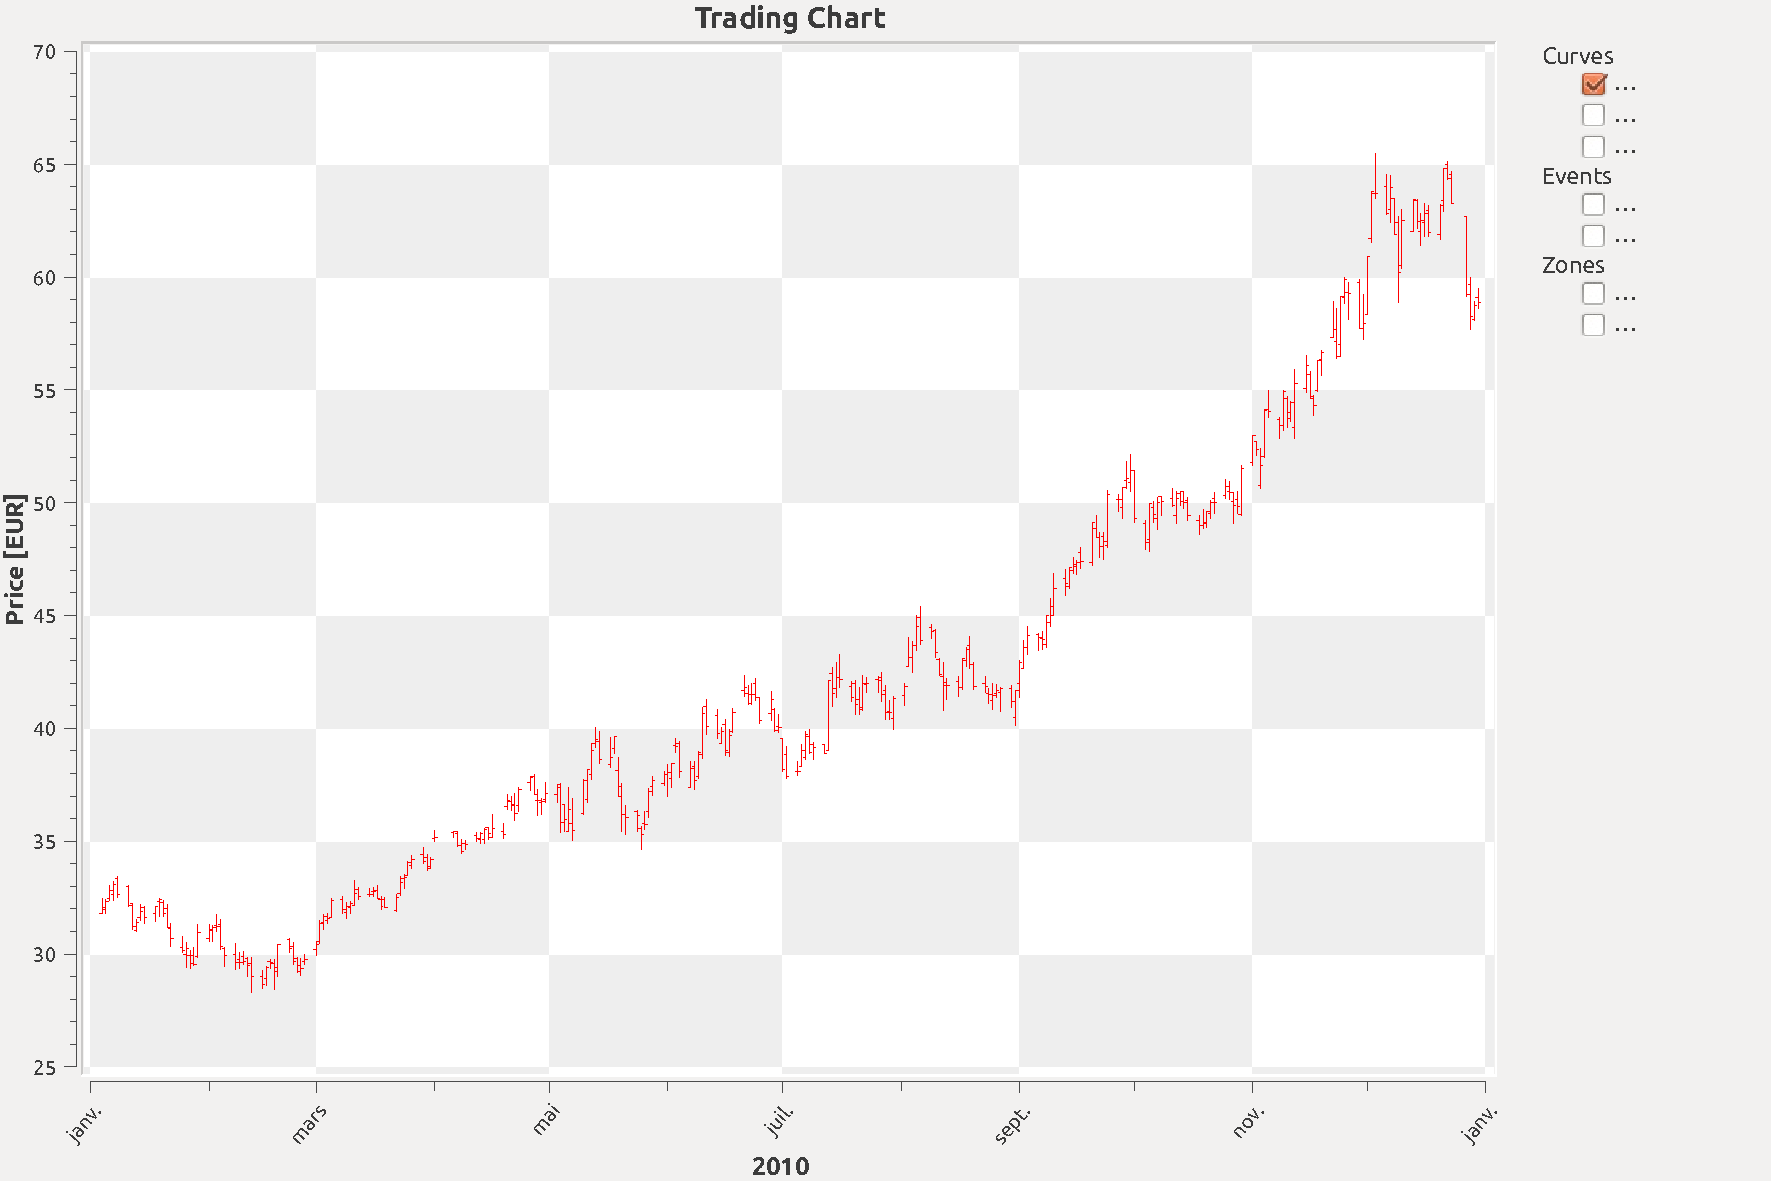
\includegraphics[scale=0.5]{stockchart.pdf}}

\subsubsection{Cash curve from Scilab man!}
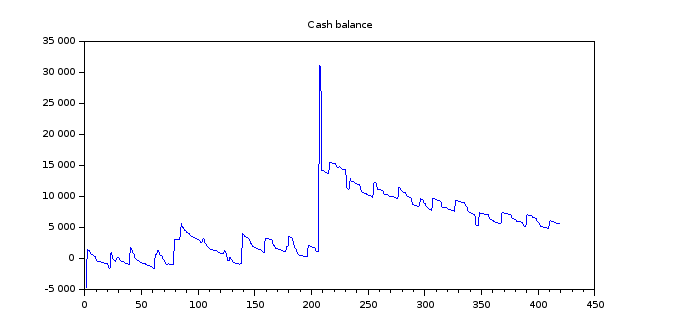
\includegraphics[scale=0.6]{Scilab-cashBalance.png}

\subsubsection{Table}
\begin{longtable}{|c|c|c|c|c|c|}
\hline
\multicolumn{6}{|c|}{Cashflows} \\
\hline
MinDate & MaxDate & Income & Charges & PnL & NumDays\\
\hline
2011-01-01 & 2021-01-13 & 83303 & 77592 & 5711 & 3665\\
\hline
2011-01-01 & 2016-10-07 & 83303 & 77592 & 5711 & 2106\\
\hline
2011-01-01 & 2016-10-06 & 83303 & 77588 & 5715 & 2105\\
\hline
2011-01-01 & 2016-10-05 & 83303 & 77581 & 5722 & 2104\\
\hline
2011-01-01 & 2016-10-04 & 83303 & 77558 & 5745 & 2103\\
\hline
2011-01-01 & 2016-10-03 & 83303 & 77484 & 5819 & 2102\\
\hline
2011-01-01 & 2016-09-30 & 83303 & 77308 & 5995 & 2099\\
\hline
2011-01-01 & 2016-09-29 & 83303 & 77278 & 6025 & 2098\\
\hline
2011-01-01 & 2016-09-28 & 83303 & 77246 & 6057 & 2097\\
\hline
2011-01-01 & 2016-09-27 & 83303 & 77223 & 6080 & 2096\\
\hline
2011-01-01 & 2016-09-26 & 82027 & 77216 & 4811 & 2095\\
\hline
2011-01-01 & 2016-09-21 & 82027 & 77134 & 4893 & 2090\\
\hline
2011-01-01 & 2016-09-20 & 82027 & 77044 & 4983 & 2089\\
\hline
2011-01-01 & 2016-09-19 & 82027 & 77018 & 5009 & 2088\\
\hline
2011-01-01 & 2016-09-16 & 82027 & 76951 & 5076 & 2085\\
\hline
 ... & ... & ... & ... & ... & ...\\
\hline
 Total &  &  &  &  & \\
\hline
\end{longtable}

To be able to have data for the drift, you need to build a C++ insert like for the kapital
go through the dates in the cashflows, and calculate a drift based on this (modulo the salary) 
\subsubsection{Graph}
%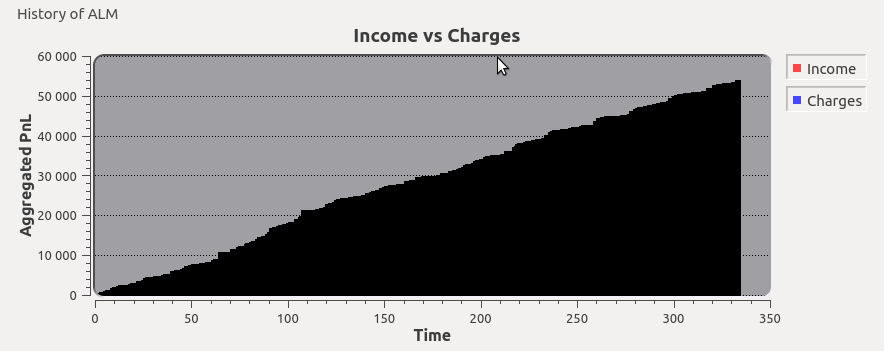
\includegraphics[width=.8\textwidth]{PnL.png}
%\begin{bchart}[min=0,max=83,step=27,unit=k\texteuro]
\bcbar[label=Income]{83}\\
\smallskip
\bcbar[label=Charges]{77}\\
\smallskip
\bcbar[label=Drift]{5}\\
\smallskip
\bcbar[label=Income]{83}\\
\smallskip
\bcbar[label=Charges]{77}\\
\smallskip
\bcbar[label=Drift]{5}\\
\smallskip
\bcbar[label=Income]{83}\\
\smallskip
\bcbar[label=Charges]{77}\\
\smallskip
\bcbar[label=Drift]{5}\\
\smallskip
\bcbar[label=Income]{83}\\
\smallskip
\bcbar[label=Charges]{77}\\
\smallskip
\bcbar[label=Drift]{5}\\
\smallskip
\bcbar[label=Income]{83}\\
\smallskip
\bcbar[label=Charges]{77}\\
\smallskip
\bcbar[label=Drift]{5}\\
\smallskip
\bcbar[label=Income]{83}\\
\smallskip
\bcbar[label=Charges]{77}\\
\smallskip
\bcbar[label=Drift]{5}\\
\smallskip
\bcbar[label=Income]{83}\\
\smallskip
\bcbar[label=Charges]{77}\\
\smallskip
\bcbar[label=Drift]{5}\\
\smallskip
\bcbar[label=Income]{83}\\
\smallskip
\bcbar[label=Charges]{77}\\
\smallskip
\bcbar[label=Drift]{6}\\
\smallskip
\bcbar[label=Income]{83}\\
\smallskip
\bcbar[label=Charges]{77}\\
\smallskip
\bcbar[label=Drift]{6}\\
\smallskip
\bcbar[label=Income]{83}\\
\smallskip
\bcbar[label=Charges]{77}\\
\smallskip
\bcbar[label=Drift]{6}\\
\smallskip
\bcbar[label=Income]{82}\\
\smallskip
\bcbar[label=Charges]{77}\\
\smallskip
\bcbar[label=Drift]{4}\\
\smallskip
\bcbar[label=Income]{82}\\
\smallskip
\bcbar[label=Charges]{77}\\
\smallskip
\bcbar[label=Drift]{4}\\
\smallskip
\bcbar[label=Income]{82}\\
\smallskip
\bcbar[label=Charges]{77}\\
\smallskip
\bcbar[label=Drift]{4}\\
\smallskip
\bcbar[label=Income]{82}\\
\smallskip
\bcbar[label=Charges]{77}\\
\smallskip
\bcbar[label=Drift]{5}\\
\smallskip
\bcbar[label=Income]{82}\\
\smallskip
\bcbar[label=Charges]{76}\\
\smallskip
\bcbar[label=Drift]{5}\\
\smallskip
\end{bchart}

%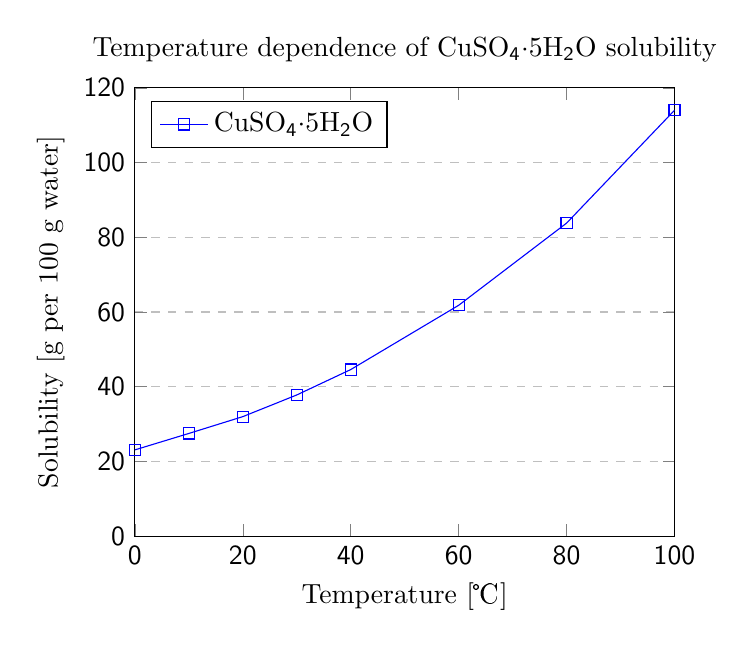
\begin{tikzpicture}
\begin{axis}[
    title={Temperature dependence of CuSO$_4\cdot$5H$_2$O solubility},
    xlabel={Temperature [\textcelsius]},
    ylabel={Solubility [g per 100 g water]},
    xmin=0, xmax=100,
    ymin=0, ymax=120,
    xtick={0,20,40,60,80,100},
    ytick={0,20,40,60,80,100,120},
    legend pos=north west,
    ymajorgrids=true,
    grid style=dashed,
]
 
\addplot[
    color=blue,
    mark=square,
    ]
    coordinates {
    (0,23.1)(10,27.5)(20,32)(30,37.8)(40,44.6)(60,61.8)(80,83.8)(100,114)
    };
    \legend{CuSO$_4\cdot$5H$_2$O}
 
\end{axis}
\end{tikzpicture}

\begin{tikzpicture}[thick,scale=1.2]
\begin{axis}[
title={Cash over time},
xlabel={Time [Days]},
ylabel={Cash [euro]},
xmin=0,xmax=0,
ymin=0,ymax=0,
xtick={0,0,0,0,0},
ytick={0,0,0,0,0},
legend pos=north west,
ymajorgrids=true,
grid style=dashed,
]
\addplot[
color=blue,
mark=*,
]
coordinates {

};
\legend{Cash}
\end{axis}
\end{tikzpicture}

\subsection{Incomes}
%Data are aggregated between Initial date: \textbf{2011/01/01} and Last date: \textbf{2021-01-13}


\subsubsection{Table}
\begin{longtable}{|c|c|c|c|c|}
\hline
\multicolumn{5}{|c|}{Cashflows} \\
\hline
Category & Debit & Credit & PnL \\
\hline
Salary & 0 & 38307 & 38307\\
\hline
Funding & 0 & 30000 & 30000\\
\hline
Sponsors & 0 & 9000 & 9000\\
\hline
Cmb & 0 & 7287 & 7287\\
\hline
Other & 0 & 2058 & 2058\\
\hline
Bank & 0 & 2056 & 2056\\
\hline
Telephone & 0 & 128 & 128\\
\hline
 ... & ... & ...\\
\hline
 Total & 77592 & 83303 & 5711 \\
\hline
\end{longtable}

\subsubsection{Graph}
\begin{bchart}[min=0,max=30,step=6,unit=k\texteuro]
\bcbar[label=Other]{30}\\
\smallskip
\bcbar[label=Salary]{19}\\
\smallskip
\bcbar[label=Sponsors]{9}\\
\smallskip
\bcbar[label=Cmb]{7}\\
\smallskip
\bcbar[label=Bank]{2}\\
\smallskip
\bcbar[label=Telephone]{0}\\
\smallskip
\end{bchart}

\subsubsection{Chart}
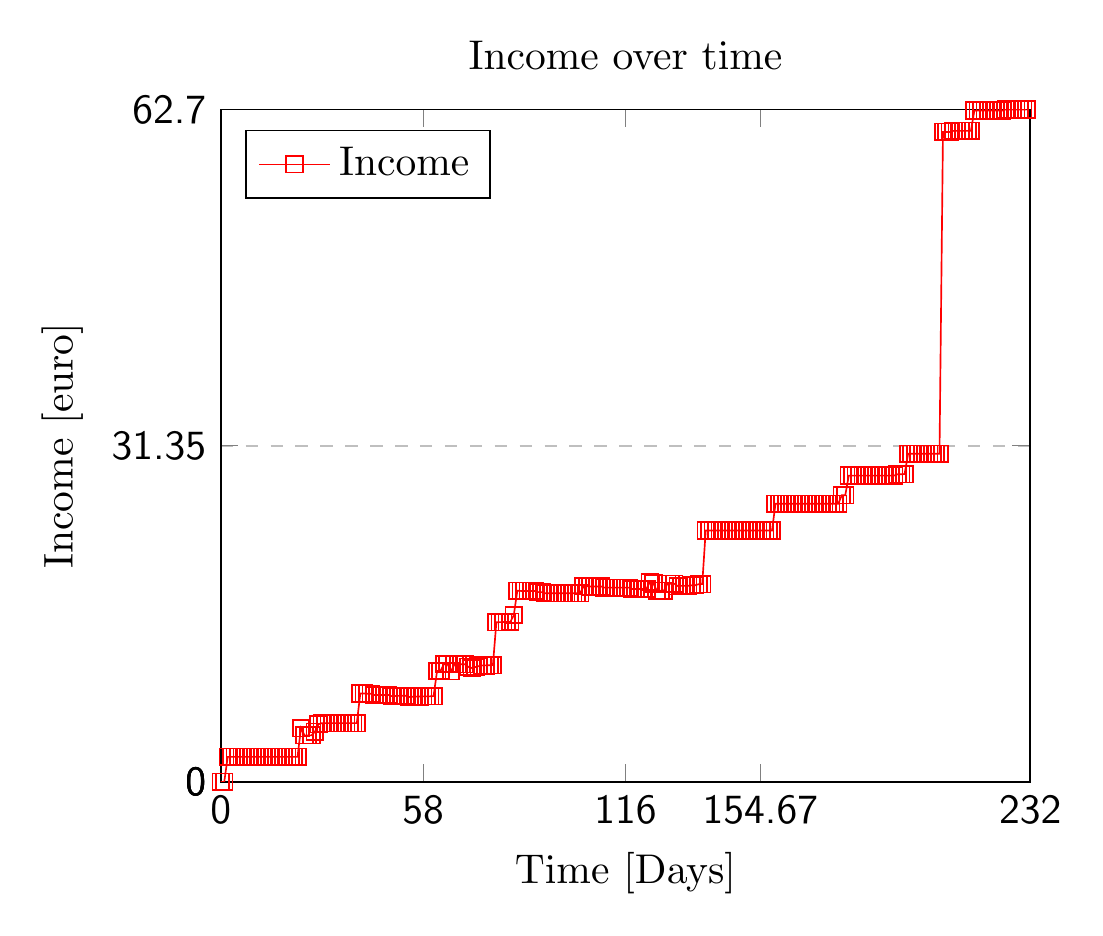
\begin{tikzpicture}[thick, scale=1.5]
\begin{axis}[
title={Income over time},
xlabel={Time [Days]},
ylabel={Income [euro]},
xmin=0,xmax=232,
ymin=0,ymax=62.704,
xtick={0,58,116,154.666666666667,232},
ytick={0,0,0,31.352,62.704},
legend pos=north west,
ymajorgrids=true,
grid style=dashed,
]
\addplot[
color=red,
mark=square,
]
coordinates {
(0,0)(1,0)(2,2.34)(3,2.34)(4,2.34)(5,2.34)(6,2.34)(7,2.34)(8,2.34)(9,2.34)(10,2.34)(11,2.34)(12,2.34)(13,2.34)(14,2.34)(15,2.34)(16,2.34)(17,2.34)(18,2.34)(19,2.34)(20,2.34)(21,2.34)(22,2.34)(23,5.015)(24,4.345)(25,4.345)(26,4.345)(27,4.68)(28,5.38)(29,5.485)(30,5.485)(31,5.485)(32,5.485)(33,5.485)(34,5.485)(35,5.485)(36,5.485)(37,5.485)(38,5.485)(39,5.485)(40,8.248)(41,8.248)(42,8.228)(43,8.228)(44,8.102)(45,8.112)(46,8.112)(47,8.112)(48,8.112)(49,8.002)(50,8.01)(51,8.026)(52,8.034)(53,8.034)(54,7.925)(55,7.941)(56,7.957)(57,7.965)(58,7.981)(59,7.981)(60,7.981)(61,8.005)(62,10.345)(63,10.345)(64,10.995)(65,10.995)(66,10.325)(67,10.975)(68,10.975)(69,10.975)(70,10.975)(71,10.724)(72,10.621)(73,10.713)(74,10.803)(75,10.865)(76,10.865)(77,10.881)(78,10.889)(79,14.889)(80,14.899)(81,14.91)(82,14.91)(83,14.916)(84,15.566)(85,17.83)(86,17.81)(87,17.81)(88,17.81)(89,17.81)(90,17.81)(91,17.7)(92,17.7)(93,17.596)(94,17.596)(95,17.596)(96,17.596)(97,17.596)(98,17.596)(99,17.596)(100,17.596)(101,17.596)(102,17.596)(103,17.596)(104,18.246)(105,18.246)(106,18.226)(107,18.226)(108,18.226)(109,18.226)(110,18.116)(111,18.116)(112,18.116)(113,18.116)(114,18.116)(115,18.116)(116,18.116)(117,18.116)(118,17.99)(119,17.99)(120,17.99)(121,17.99)(122,17.99)(123,18.64)(124,18.497)(125,17.827)(126,17.827)(127,17.827)(128,18.477)(129,18.477)(130,18.477)(131,18.264)(132,18.28)(133,18.28)(134,18.288)(135,18.334)(136,18.342)(137,18.44)(138,18.448)(139,23.448)(140,23.448)(141,23.448)(142,23.448)(143,23.448)(144,23.448)(145,23.448)(146,23.448)(147,23.448)(148,23.448)(149,23.448)(150,23.448)(151,23.448)(152,23.448)(153,23.448)(154,23.448)(155,23.448)(156,23.448)(157,23.448)(158,23.448)(159,25.937)(160,25.937)(161,25.937)(162,25.937)(163,25.937)(164,25.937)(165,25.937)(166,25.937)(167,25.937)(168,25.937)(169,25.937)(170,25.937)(171,25.937)(172,25.937)(173,25.937)(174,25.937)(175,25.937)(176,25.937)(177,25.937)(178,26.737)(179,26.737)(180,28.562)(181,28.562)(182,28.562)(183,28.562)(184,28.562)(185,28.562)(186,28.562)(187,28.562)(188,28.562)(189,28.562)(190,28.562)(191,28.562)(192,28.562)(193,28.565)(194,28.685)(195,28.693)(196,28.709)(197,30.605)(198,30.605)(199,30.605)(200,30.605)(201,30.605)(202,30.605)(203,30.605)(204,30.605)(205,30.605)(206,30.605)(207,60.605)(208,60.605)(209,60.605)(210,60.704)(211,60.704)(212,60.704)(213,60.704)(214,60.704)(215,60.704)(216,62.595)(217,62.6)(218,62.6)(219,62.6)(220,62.6)(221,62.6)(222,62.6)(223,62.6)(224,62.6)(225,62.704)(226,62.704)(227,62.704)(228,62.704)(229,62.704)(230,62.704)(231,62.704)
};
\legend{Income}
\end{axis}
\end{tikzpicture}

%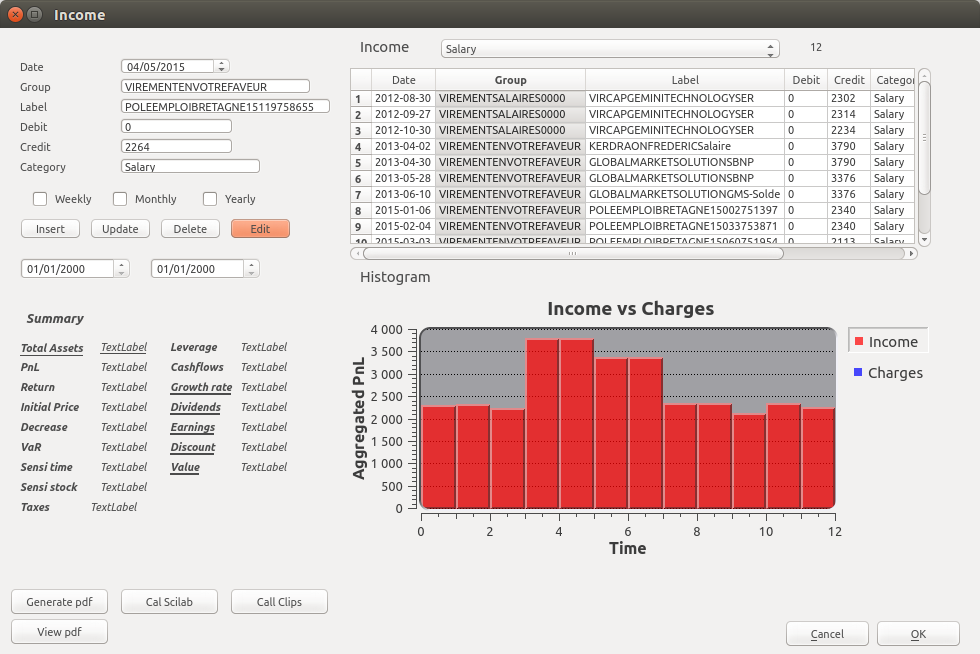
\includegraphics[width=.8\textwidth]{Income.png}

\subsection{Charges}
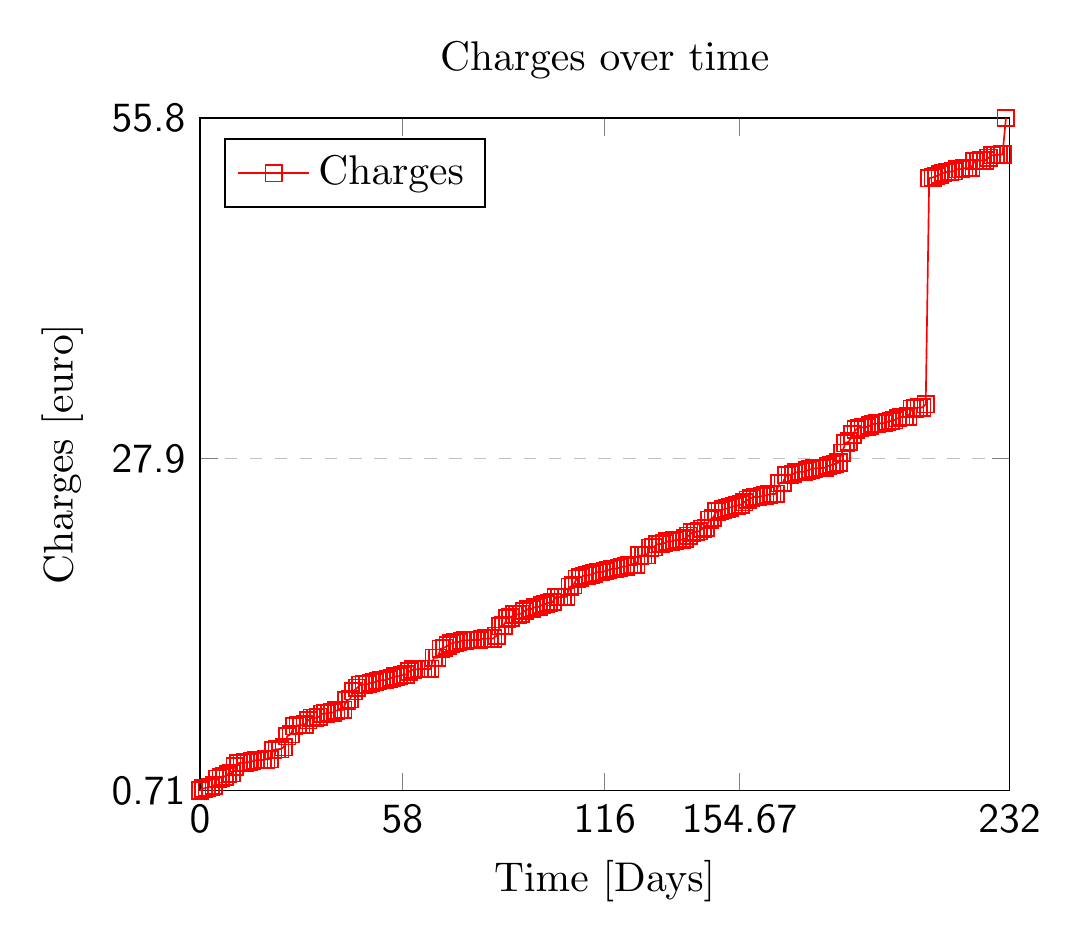
\begin{tikzpicture}[thick, scale=1.5]
\begin{axis}[
title={Charges over time},
xlabel={Time [Days]},
ylabel={Charges [euro]},
xmin=0,xmax=232,
ymin=0.713,ymax=55.799,
xtick={0,58,116,154.666666666667,232},
ytick={0.713,0.3565,0,27.8995,55.799},
legend pos=north west,
ymajorgrids=true,
grid style=dashed,
]
\addplot[
color=red,
mark=square,
]
coordinates {
(0,0.713)(1,0.878)(2,0.94)(3,0.98)(4,1.117)(5,1.664)(6,1.783)(7,1.85)(8,2.055)(9,2.116)(10,2.669)(11,2.955)(12,2.973)(13,2.998)(14,3.033)(15,3.103)(16,3.181)(17,3.201)(18,3.215)(19,3.258)(20,3.278)(21,4.013)(22,4.097)(23,4.105)(24,4.251)(25,5.155)(26,5.313)(27,5.97)(28,6.048)(29,6.048)(30,6.122)(31,6.461)(32,6.66)(33,6.66)(34,6.74)(35,6.995)(36,7.019)(37,7.079)(38,7.088)(39,7.265)(40,7.289)(41,7.316)(42,8.087)(43,8.188)(44,8.84)(45,9.108)(46,9.362)(47,9.398)(48,9.421)(49,9.522)(50,9.574)(51,9.69)(52,9.753)(53,9.753)(54,9.838)(55,9.95)(56,10.046)(57,10.079)(58,10.145)(59,10.205)(60,10.459)(61,10.61)(62,10.632)(63,10.665)(64,10.665)(65,10.665)(66,10.665)(67,11.577)(68,11.581)(69,12.312)(70,12.41)(71,12.582)(72,12.747)(73,12.837)(74,12.863)(75,12.983)(76,13.006)(77,13.028)(78,13.036)(79,13.036)(80,13.036)(81,13.139)(82,13.153)(83,13.154)(84,13.154)(85,13.384)(86,14.169)(87,14.218)(88,14.795)(89,14.883)(90,15.122)(91,15.132)(92,15.192)(93,15.413)(94,15.557)(95,15.577)(96,15.727)(97,15.747)(98,15.905)(99,15.985)(100,16.086)(101,16.15)(102,16.545)(103,16.56)(104,16.56)(105,16.576)(106,17.385)(107,17.531)(108,18.064)(109,18.159)(110,18.307)(111,18.323)(112,18.396)(113,18.492)(114,18.592)(115,18.592)(116,18.672)(117,18.776)(118,18.857)(119,18.869)(120,18.944)(121,19.03)(122,19.048)(123,19.177)(124,19.185)(125,19.185)(126,19.96)(127,19.988)(128,19.996)(129,20.585)(130,20.653)(131,20.873)(132,20.899)(133,20.959)(134,21.103)(135,21.103)(136,21.193)(137,21.233)(138,21.241)(139,21.341)(140,21.575)(141,21.84)(142,21.886)(143,21.947)(144,22.151)(145,22.212)(146,22.885)(147,23.029)(148,23.558)(149,23.62)(150,23.731)(151,23.807)(152,23.897)(153,23.987)(154,24.049)(155,24.129)(156,24.33)(157,24.519)(158,24.652)(159,24.756)(160,24.757)(161,24.822)(162,24.873)(163,24.953)(164,24.995)(165,25.004)(166,25.888)(167,25.904)(168,26.531)(169,26.561)(170,26.641)(171,26.773)(172,26.808)(173,26.813)(174,26.919)(175,27.012)(176,27.096)(177,27.104)(178,27.126)(179,27.136)(180,27.289)(181,27.389)(182,27.465)(183,27.571)(184,28.377)(185,29.166)(186,29.301)(187,29.862)(188,30.271)(189,30.429)(190,30.462)(191,30.48)(192,30.601)(193,30.735)(194,30.764)(195,30.787)(196,30.803)(197,30.915)(198,30.975)(199,31.052)(200,31.204)(201,31.305)(202,31.317)(203,31.353)(204,31.987)(205,32.005)(206,32.078)(207,32.086)(208,32.342)(209,50.869)(210,50.925)(211,51.035)(212,51.166)(213,51.295)(214,51.368)(215,51.402)(216,51.43)(217,51.595)(218,51.613)(219,51.683)(220,51.694)(221,51.699)(222,52.251)(223,52.299)(224,52.316)(225,52.321)(226,52.546)(227,52.75)(228,52.77)(229,52.787)(230,52.808)(231,55.799)
};
\legend{Charges}
\end{axis}
\end{tikzpicture}


\subsubsection{Charges plot}
Removed to preserve my eyes from the colors....!!!!\\
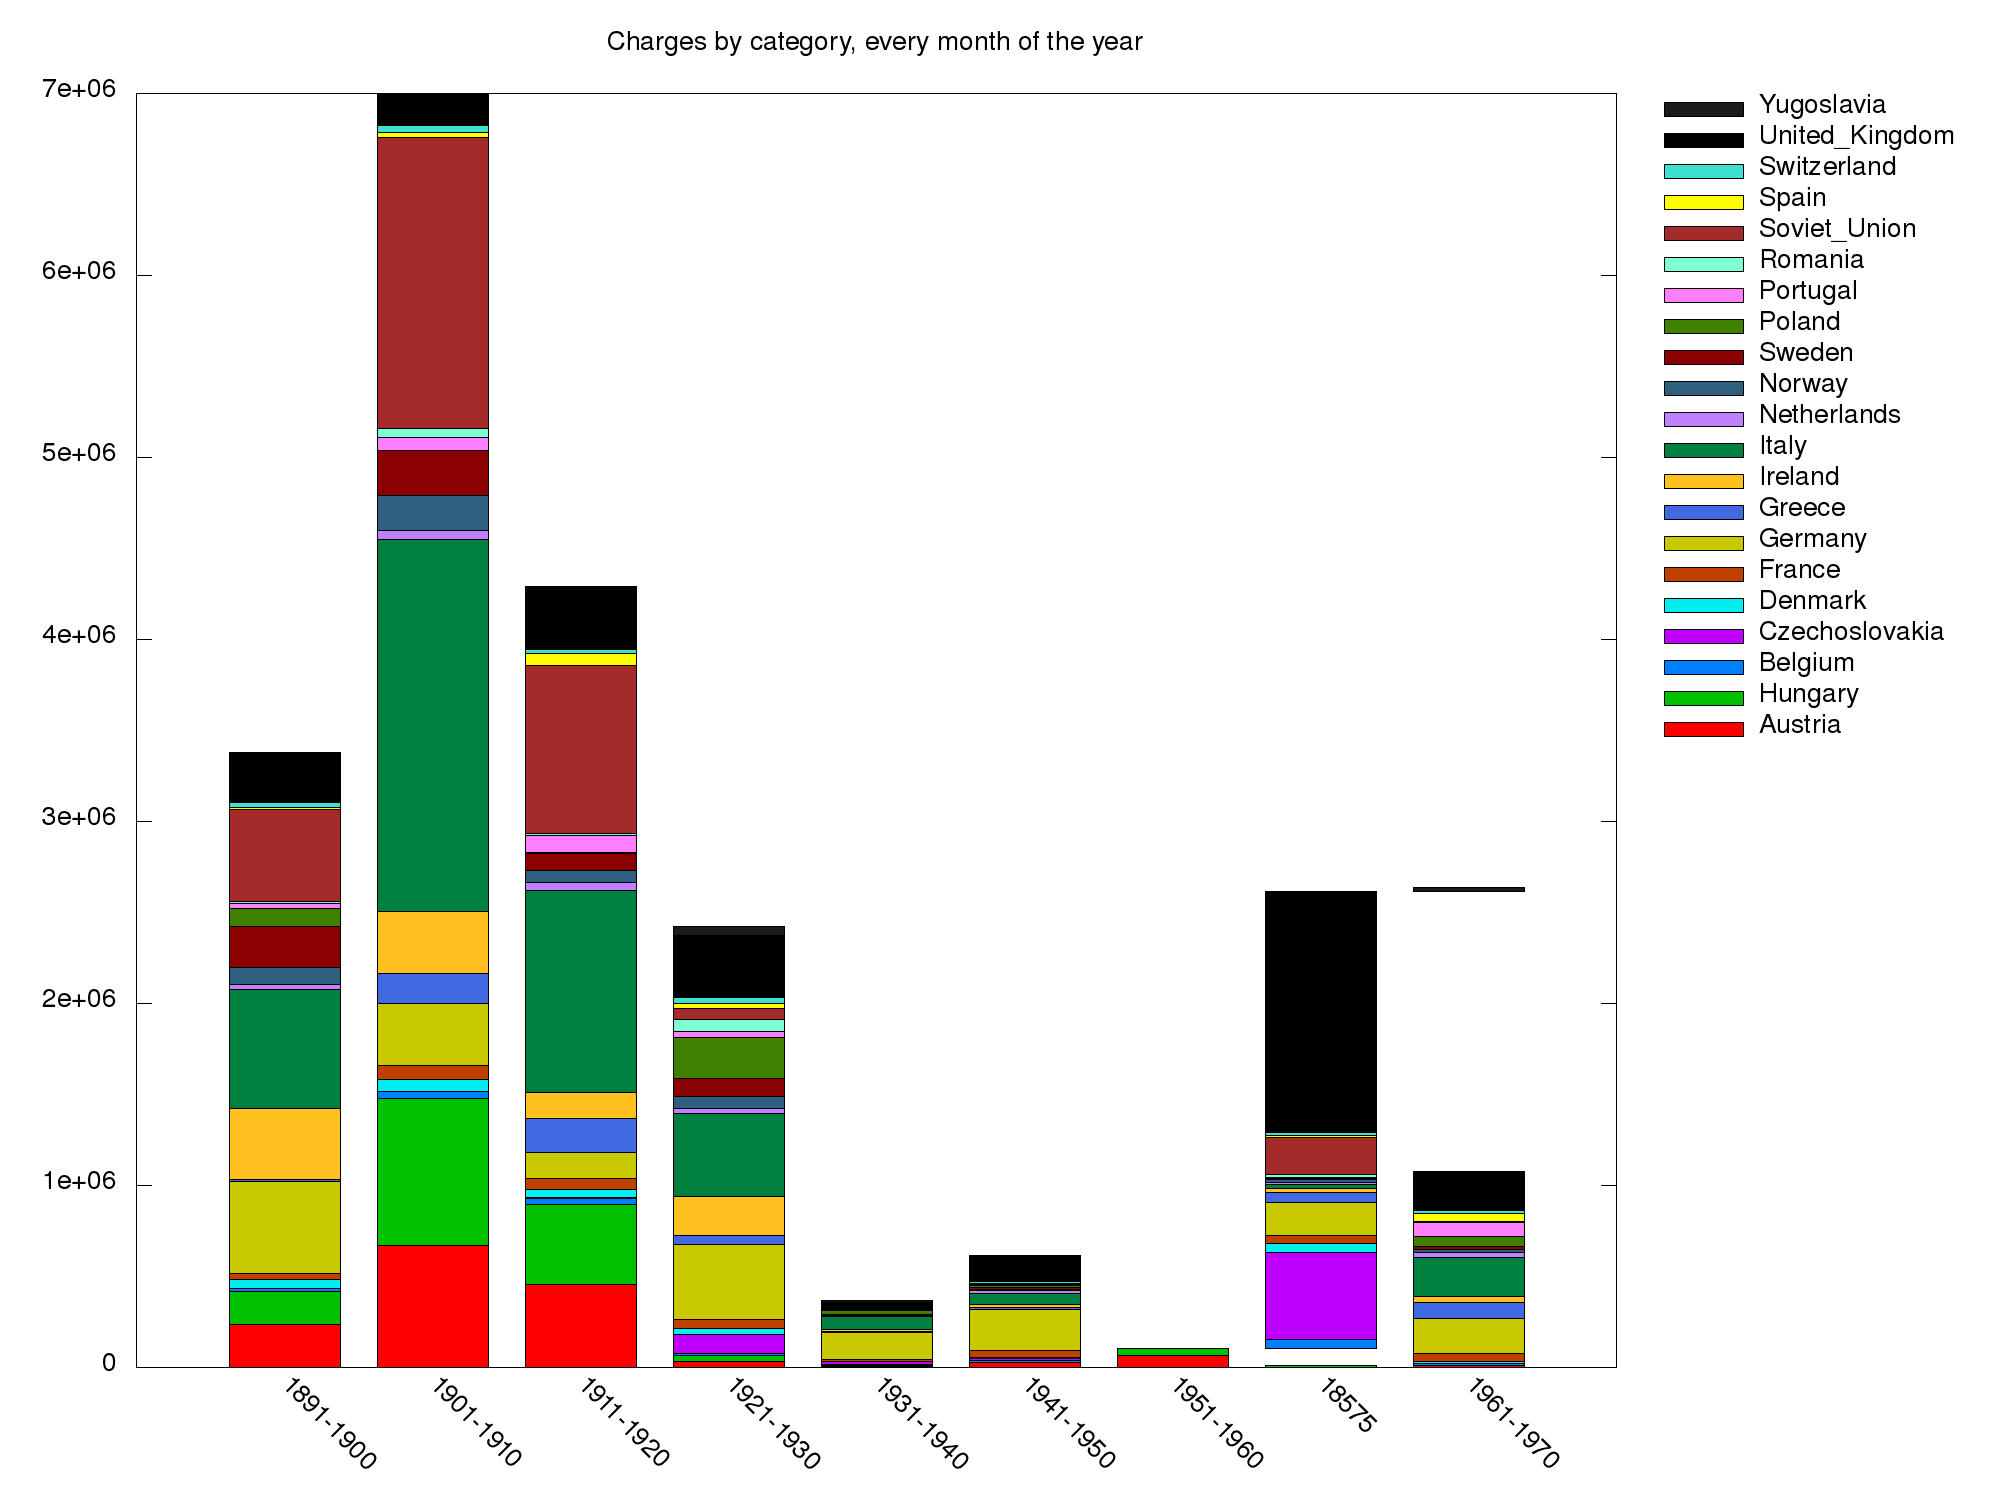
\includegraphics[scale=0.3]{Charges2.png}

\subsubsection{Charges kiviat}
%One note :-) This should be random!
\begin{tikzpicture}[scale=0.5]
\tkzKiviatDiagramFromFile[
        scale=.5,
        label distance=.5cm,
        gap     = 1,
        label space=3,  
        lattice = 10]{chargesKiviat.dat}
\tkzKiviatLineFromFile[thick,
                       color      = blue,
                       mark       = ball,
                       ball color = blue,
                       mark size  = 4pt,
                       fill       = blue!20]{chargesKiviat.dat}{2}
\tkzKiviatLineFromFile[thick,
                       color      = red,
                       mark       = ball,
                       ball color = red,
                       mark size  = 4pt,
                       fill       = red!20]{chargesKiviat.dat}{1}     
\end{tikzpicture}


\subsubsection{Table}
\begin{longtable}{|c|c|c|c|c|}
\hline
\multicolumn{5}{|c|}{Cashflows} \\
\hline
Category & Debit & Credit & PnL \\
\hline
Cmb & 7201 & -963 & -8164\\
\hline
Debt & 19965 & 0 & -19965\\
\hline
Bank & 8527 & 0 & -8527\\
\hline
Other & 8205 & 0 & -8205\\
\hline
Cash & 4330 & 0 & -4330\\
\hline
Food & 2487 & 0 & -2487\\
\hline
Toxics & 2395 & 0 & -2395\\
\hline
Rent & 1066 & 0 & -1066\\
\hline
Telephone & 669 & 0 & -669\\
\hline
Energy & 448 & 0 & -448\\
\hline
Home & 272 & 0 & -272\\
\hline
Health & 232 & 0 & -232\\
\hline
Transport & 2 & 0 & -2\\
\hline
 ... & ... & ... & ...\\
\hline
 Total & 55799 & 62704 & 6905 \\
\hline
\end{longtable}


\subsubsection{Graph}
\begin{bchart}[min=0,max=21,step=4,unit=k\texteuro]
\bcbar[label=Bank]{8}\\
\smallskip
\bcbar[label=Boat]{0}\\
\smallskip
\bcbar[label=Car]{0}\\
\smallskip
\bcbar[label=Cash]{7}\\
\smallskip
\bcbar[label=Cmb]{6}\\
\smallskip
\bcbar[label=Debt]{21}\\
\smallskip
\bcbar[label=Energy]{0}\\
\smallskip
\bcbar[label=Food]{7}\\
\smallskip
\bcbar[label=Health]{0}\\
\smallskip
\bcbar[label=Home]{0}\\
\smallskip
\bcbar[label=Other]{13}\\
\smallskip
\bcbar[label=Rent]{2}\\
\smallskip
\bcbar[label=Telephone]{1}\\
\smallskip
\bcbar[label=Toxics]{5}\\
\smallskip
\bcbar[label=Transport]{0}\\
\smallskip
\end{bchart}


\subsubsection{Chart}

\subsubsection{Cheese}
\begin{tikzpicture}[scale=2]
\foreach \p/\t in {
10 / Bank-8.111k\texteuro ,
0 / Boat-0.28k\texteuro ,
1 / Car-0.918k\texteuro ,
9 / Cash-7.231k\texteuro ,
8 / Cmb-6.866k\texteuro ,
27 / Debt-21.209k\texteuro ,
0 / Energy-0.489k\texteuro ,
10 / Food-7.962k\texteuro ,
0 / Health-0.517k\texteuro ,
0 / Home-0.451k\texteuro 
17 / Other-13.551k\texteuro 
3 / Rent-2.582k\texteuro 
1 / Telephone-1.073k\texteuro 
7 / Toxics-5.635k\texteuro 
0 / Transport-0.717k\texteuro 
}
  {
\setcounter{a}{\value{b}}
\addtocounter{b}{\p}
\slice{\thea/100*360}
          {\theb/100*360}
          {\p\%}{\t}
  }
\end{tikzpicture}


%%%%%%%%%%%%%%%%%%%%%%%%%%%%%%%%%%%%%%%%%%%%%%%%%%%%%%%%%%%%%%%%%%%%%%%%%%%%%%%%%%%%%%%%%%%%%%%%%%%%%%%%%%%%%%%%%%%%%%%%%%%%%%%%%%%%%%%%%%%%%%%%%%%%%%%%%%%%%%

\end{document}

